\documentclass[a4paper,11pt]{article}
\usepackage[finnish]{babel}

\usepackage{amsmath}
\usepackage[utf8]{inputenc}
\usepackage[T1]{fontenc}
\usepackage{parskip}
\usepackage{csquotes}
\usepackage{graphicx}

\usepackage{amsmath}
\usepackage{amssymb}
\usepackage{eurosym}
\usepackage{tyyli}

\usepackage[backend=biber,style=numeric]{biblatex}
\addbibresource{viitteet.bib}

\begin{document}

{
\thispagestyle{empty}
{\large
\textbf{Helsingin yliopisto}
\par
MAST31901 - History of Mathematics
}

\vspace{7cm}

{\huge
Kurssiessee:}
\par
{\Large \bf Euler ja lukuteoria}

\vspace{2cm}

{\Large Elli Kiiski}

\vfill

{\large \today}
}

\clearpage

\pagenumbering{arabic}

\section{Johdanto}

On hankala päättää millä titteleillä hänet esittelisi; ainoastaan hänen ansioluettelonsa läpikäyminen vaatisi oman kymmensivuisen esseensä. Tällä kertaa tarkoitusperiimme kuitenkin sopii tituleerata tätä yleisneroa matemaatikko Leonhard Euleriksi.

Määrittelyongelmat eivät tosin jää siihen, sillä Euler onnistui tuottamaan mullistavia tuloksia myös ällistyttävän monella eri osa-alueella matematiikan alan sisällä. Poistamme hetkeksi mielestämme maailman kauneimman yhtälön\footnote{Eulerin identiteettiä $e^{\pi i}+1=0$ on verrattu Shakespearin sonettin ja testattu maailman kauneimmaksi yhtätlöksi jopa magneettikuvaustutkimuksilla! \cite{identity}} sekä Königsbergin siltaongelman\footnote{Euler todisti, ettei Königsbergissä (nykyinen Kaliningrad) ollut mahdollista tehdä kävelyretkeä, jolla ylittää kunkin kaupungin seitsemästä sillasta täsmälleen kerran \cite{silta}} ja keskitymme tällä erää matematiikan kuningattareen\footnote{\enquote{Mathematics is the queen of the sciences and number theory is the queen of mathematics.}\\Carl Friedrich Gauss \cite{quotes}}, lukuteoriaan. Eulerin saavutukset yksin tällä sektorilla olisivat varmasti riittäneet nostamaan hänet historiankirjoihin yhtenä historian suurimmista matemaatikoista.

Yhtäläisesti historiallisena kuin matemaattisenakin esseenä tasapainottelemme näiden näkökulmien välillä varoen uppoutumasta liian syvällisesti kumpaankaan. Toisaalta pyrkimyksenä on koota yhteen johdonmukainen\footnote{Varoituksen sananen alaviitteistä: Johtuen kirjoittajan rönsyilevästä ajatuksenkulusta (ja pakonomaisesta tarpeesta selittää kaikki auki) lukijan on syytä varautua ylenpalttiseen määrään lisähuomautuksia, tarkennuksia ja hauskoja faktoja, jotka voi halutessaan myös tyystin sivuuttaa.} kuva Eulerin lukuteoreettisesta elämäntyöstä niin ajallisessa kuin matemaattisessakin kontekstissa. Se kaikki alkaa jo hyvän aikaa ennen Eulerin syntymää.

\section{Lukuteoria ennen Euleria}
\label{kakkoi}

Oikeastaan vielä Eulerinkaan aikana ei puhuttu matematiikan alasta nimeltä lukuteoria \cite{Karatsuba}. Kuitenkin ongelmia, joiden katsotaan nykyään kuuluvan lukuteorian piiriin, on ratkottu paljon ennen ajanlaskumme alkua. Ensimmäisenä todisteena pidetään babylonialaista Plimpton 322 savitaulua, joka sisältää vaikuttavan määrän yhtälön $a^2+b^2=c^2$ toteuttavia lukukolmikoita, joita kutsutaan tätä nykyä Pythagoraan kolmikoiksi.

Juuri Pythagoraan (n. 580–500 eaa.) nimissä olevat löydökset, joihin kuuluu noiden kolmikoiden ja niihin liittyvän Pythagoraan lauseen lisäksi mm. monikulmioluvut kuten kolmio- ja neliöluvut, ovat ensimmäisiä merkkejä lukujen teoreettisemmasta tutkimisesta \cite{Burton}. Myös myöhemmin tutuksi tulevat täydelliset luvut (\textit{engl. perfect number}) ja ystävälliset lukuparit (\textit{engl. amicable numbers}) yhdistetään häneen ja aikalaisiin seuraajiinsa.

Antiikin Kreikan toinen suuri matemaatikko Euklides (n. 300 eaa.) tunnetaan etenkin vaikuttavasta\footnote{Mitä vähättelyä! \textit{Elements} oli aikansa ensimmäinen (tähän päivään säilynyt) matemaattiseen päättelyyn perustuva teos. Euklides käytännössä keksi geometrian.} teoksessaan \textit{Elements} \cite{Elements}, joka käsittelee pääosin geometriaa. Sen kirjoissa VII ja IX esitellään kuitenkin perustavanlaatuisia lukuteorian tuloksia etenkin alkulukuihin liittyen. Merkittävimpiin poimintoihin kuuluvat mm. Euklideen algoritmi (suurimman yhteisen tekijän\footnote{Luku $d$ on positiivisten kokonaislukujen $a$ ja $b$ suurin yhteinen tekijä, jos sekä $a$ että $b$ ovat sillä jaollisia ja jokainen molemmat luvut jakava toinen luku jakaa myös luvun $d$. Tätä merkitään $d=\text{syt}(a,b)$.} löytäminen) ja todistus alkulukujen määrän äärettömyydestä. Euklides todisti myös Eulerin myöhemmin täydentämän lauseen

\begin{center}
    \textit{Jos luku $a$ on muotoa $(2^p-1)2^{p-1}$, missä sekä $p$ että $2p-1$ ovat alkulukuja, $a$ on täydellinen\footnote{Täydellinen luku määritellään ihan pian luvussa \ref{kolmoi}.}.}
\end{center}

Maanmiestensä tapaan antiikin Kreikan lopputaipaleen aikaan\footnote{Diofantoksen synnyin- tai kuolinaikaa ei tiedetä edes vuosikymmenen tarkkuudella. Persoonana hänestä ei ylipäätään tiedetä juuri erästä nokkelaa runonpartta enempää: \enquote{\textit{His boyhood lasted for $\frac{1}{6}$ of his life; his beard grew after $\frac{1}{12}$ more; after $\frac{1}{7}$ more he married, and his son was born five years later; the son lived to half his father’s age and the father died four years after his son.}}\cite{Burton}  Arvoitusta vastaavan yhtälön $x=\frac{1}{6}x+\frac{1}{12}x+\frac{1}{7}x+5+\frac{1}{2}x+4$ ratkaisemalla voidaan sentään laskea Diofantoksen iäksi 84 vuotta.} elänyt Diofantos (n. 250 jaa.) antoi panoksensa lukuteorialle. Jos Euklides oli geometrian isä, voidaan Diofantosta puolestaan pitää algebran keksijänä. Lukuteorian saralla hänet tunnetaan kuitenkin parhaiten hänen mukaansa nimetyistä kokonaislukukertoimisista yhtälöistä, joissa on vähintään kaksi tuntematonta ja joihin etsitään kokonaislukuratkaisuja. Esimerkiksi $a^2+b^2=c^2$ on Diofantoksen yhtälö, kun sen rarkaisuksi etsitään Pythagoraan kolmikkoa.

Seuraavilta vuosisadoilta näyttää puuttuvan kaikki nimekkäät lukuteoreetikot, joiden löydökset ja keksinnöt olisivat tulleet laajalle yleisölle tutuksi. Näkökanta on kuitenkin varsin Eurooppa-keskeinen. Nimittäin noina aikoina esimerkiksi Intiassa kehitettiin nykyinen kantalukujärjestelmä sekä otettiin muita edistysaskelia, eikä islamilaisenkaan maailman panosta ole syytä väheksyä. Kuitenkaan Brahmaguptan\footnote{Brahmagupta (n. 600 jaa.) edeltäjänsä Āryabhaṭan jalanjäljissä löysi ensimmäisenä yleisen rakaisun lineaariselle Diofantoksen yhtälölle $ax+bx=c$. Oikeastaan nämä intialaiset matemaatikot olivat tosiasiassa ne, jotka hyväksyivät Diofantoksen yhtälön ratkaisuksi vain kokonaislukuja. Diofantos itse oli ollut kiinnostunut kaikista rationaalilukuratkaisuista, vaikka määritelmä kantaakin hänen nimeään.\cite{Burton}} tai Thābit ibn Qurran\footnote{Thābit ibn
Qurra (n. 836–901) oli paitsi taitava kääntäjä (hän käänsi useita antiikin Kreikan teoksia arabiaksi) myös hänen oma kirjansa \textit{Book on the Determination of Amicable Numbers} esitteli säännön, jolla voi generoida ystävällisiä lukupareja (jos alaviitteellä voisi olla alaviite, kirjoittaisin auki myös kyseisen säännön). Hänen nimissään ei kuitenkaan ole yhtään löydettyä paria.} kaltaiset nimet eivät esiinny historian kirjoissamme yhtä tiuhaan.

Matematiikan kiinnostus oli ylipäätään ollut vähäistä 1500-luvulla, mutta pian vuosisadan vaihtuessa lukuteorian osalta alaa alkoi elvyttää Pierre de Fermat (1601–1665). Mieleepainuvin häneen yhdistetty seikka lienee \enquote{ihmeellinen todistus}, jonka hän väittää keksineensä Fermat'n suurelle lauseelle\footnote{Fermat'n suuri lause löydettiin hänen jo kuoltua raapustettuna Diofantoksen \textit{Arithmetican} marginaaliin yhdessä (vapaasti suomennetun) huomautuksen \enquote{Olen keksinyt tälle ihmeellisen todistuksen, joka ei kuitenkaan mahdu tähän marginaaliin} kera. Lause onnisttiin todistamaan vasta vuonna 1995. Andrew Wiles käytti ratkaisussaan varsin modernia matematiikkaa, mikä vahvasti vihjaa siihen suuntaan, ettei Fermatilla tainnutkaan olla tiedossaan virheetöntä todistusta.} (\textit{engl. Fermat's last theorem}), jonka mukaan mitkään positiiviset kokonaisluvut $a$, $b$ ja $c$ eivät toteuta yhtälöä $a^n+b^n=c^n$, kun $n>2$. Moneen muuhunkaan Fermat'n teoreemaan ei ole löydetty hänen omia todistuksiaan (joskin hän ne väitti todistaneensa), mutta myöhemmin muiden näytettyä niitä päteviksi\footnote{Luku \ref{neloi} käsittelee Euleri Fermat'n töiden jatkajana. Lisää myös Fermat'sta silloin.} ne kantavat silti keksijänsä nimeä.

Vuihdoin vonna 1707 syntyi Leonhard Euler, joka seuraavana 76 elinvuotenaan kehitti eteenpäin (lähes) jokaisen aikaansa edeltäneen lukuteoreetikon aikaansaannoksia.

\section{Täydelliset luvut ja ystävälliset parit}
\label{kolmoi}

Kuten todettu, tuottoisana matemaatikkona Euler ehti tuottaa lukuisia löytöjä ja todistuksia myös lukuteorian saralla. Vaikka monimutkaisimmat näistä saavat $n$. vuoden matematiikan opiskelijankin raapimaan päätään, osa puolestaan vaikuttaa nykyihmiselle hyvinkin yksinkertaisilta. Kansantajuisimmasta päästä ovat niin kutsutut täydelliset luvut ja ystävälliset lukuparit.

\begin{center}
    \textbf{Täydellinen luku} \textit{Positiivinen kokonaisluku, joka on omien itseään pienempien tekijöidensä summa. \textit{Esimerkiksi} luku $6$ on täydellinen, koska $1+2+3=6$.}
\end{center}

Palataan nyt aiemmin luvussa \ref{kakkoi} esiteltyyn Euklideen täydellisiä lukuja koskevaan lauseeseen, jonka Euler todisti omana aikanaan pätevän myös toiseen suuntaan. Hänen versionsa kuuluu seuraavasti.

\begin{center}
    \textit{Jos luku $a$ on parillinen täydellinen luku se voidaan kirjoittaa muodossa $(2^p-1)2^{p-1}$, missä sekä $p$ että $2p-1$ ovat alkulukuja.}
\end{center}

Euler siis todisti, että Euklideen todistama yhteys täydelliseten lukujen ja lausekkeen $(2^p-1)2^{p-1}$ välillä on yhtäpitävä eli pätee molempiin suuntiin. Siinä missä Euklides näytti, että luvun toteuttaessa kyseisen lausekkeen, se on täydellinen, Euler osoitti, että luvun ollessa täydellinen ja parillinen (parittomia täydellisiä lukuja ei ole löydetty tai niiden olemassaolemattomuutta todistettu \ref{lähde}) se toteuttaa kyseisen lausekkeen.

Ystävälliset lukuparit liittyvät läheisesti täydellisiin lukuihin, tavallaan tällaisten lukujen voisi luonnehtia olevan ikään kuin täydellisiä toisilleen. Täsmällinen määritelmä voidaan kirjoittaa seuraavanlaisesti.

\begin{center}
    \textbf{Ystävällinen lukupari} \textit{Pari $(A, B)$ erisuuria positiivisia kokonaislukuja, joille pätee, että luvun $A$ itseään pienempien tekijöiden summa on $B$ sekä toisinpäin. \textit{Esimerkiksi} $(220, 284)$ on tällainen.}
\end{center}

Ennen Euleria ystävällisiä lukupareja oli löydetty vasta kaksi, niin kutsutut Pythagoraan pari $(220, 284)$ sekä Fermat-Descartesin pari $(17296, 18416)$. Euler kasvatti tätä määrää huimalla 59 parilla, joiden joukossa on myös parittomia lukupareja. Esimerkiksi $(67095=3^3\cdot5\cdot7\cdot71, 71145=3^3\cdot5\cdot17\cdot31)$ on Eulerin löytämä pariton ystävällinen lukupari.

Ystävällisiä lukupareja tunnetaan nykyään yli miljardi, ja niistä suurimmat ovat tuhansia numeroita pitkiä. Tietokoneiden laskentatehon kehityksellä on tietenkin ollut tähän valtava vaikutus, ja uusien löytöjen algoritmista generointia voi tuskin verrata Eulerilla käytössään olleisiin metodeihin. Tutkimalla lukujen ominaisuuksia Euler kuitenkin huomasi alkuluvuilla olevan hyödyllisiä ominaisuuksia tekijöiden summia laskettaessa, joita hän pystyi käyttämään hyväkseen. \cite{tarvii kaivaa siitä yhdestä exam paperista} % ja tää on ehk vähän huono muutenkin, tähän vois kirjottaa jotain Euler's rulesta ja sen edeltäjästä Thābit ibn Qurran keksimästä, mut en kyl nyt tiedä onko niiden avulla löydetty tyyliin ku pari tai jotain XD

Loppujen lopuksi onkin vähemmän merkittävää, kuinka monta uutta ystävällistä lukuparia tai täydellistä lukua Euler itse onnistui löytämään. Hänen kehittämänsä menetelmät niiden tuottamiseen sen sijaan ovat antaneet työkaluja tulevaisuuden matemaatikoille kasvattaa kyseisiä lukulistoja.

\section{Eulerin $\varphi$-funktio ja muita nimikkotuotteita}
\label{neloi}

Siltä varalta, ettei Eulerin massiivista aikaansannosten määrää ole vielä alleviivattu tarpeeksi, päästään kyseiseen tavoitteeseen viimeistään tutkimalla Wikipedia-sivua \textit{List of things named after Leonhard Euler} (lista Leonhard Eulerin mukaan nimetyistä asioista) \cite{listofthings}. Pelkästään teoreemoja hänen nimellään löytyy 11 kappaletta. Listalle niin ikään lukeutuva Eulerin identiteetti vilahtikin jo erässä aiemmassa alaviitteessä, mutta listaus sisältää tietysti myös useita merkittäviä lukuteorian tuloksia.

Eulerin vuonna 1763 esittelemä $\varphi$-funktio (\textit{engl. Euler's totient function}) \cite{totient} on eräs lukuteoriassa usein näyttäytyvistä (ja ehkä myös yksi kiinnostavimmista\footnote{Kirjoittaja sattui tekemään kandityönsä \textit{The Order of Euler's totient function} kyseisen funktion kasvuvauhdin alarajasta \cite{kandi}.}) funktioista. Sen arvo kertoo lukujen jaollisuudesta, tosin käänteisesti: mitä useammalla luvulla jaollinen luku kokoonsa nähden on, sitä pienempi on $\phi$-funktion arvo.

\begin{center}
    \textbf{Eulerin $\phi$-funktio $\phi: \N \rightarrow \N$}\\
    \textit{$\phi(1)=1$ sekä kaikilla $n\geq2$, $\phi(n)$ on sellaisten lukujen $1,2,...,n$ määrä, joiden suurin yhteinen tekijä luvun $n$ kanssa on $1$.}
\end{center}

Eulerin $\phi$-funktiota käytetään laajasti lukuteoriassa ja jopa käytännön sovelluksissa, kuten luvussa \ref{seiska} kuuullaan. 

Myös lukuteorian todistuksissa toisinaan esiintyvä Eulerin-Macheronin vakio $\gamma\approx0,5772$ kantaa päähenkilömme nimeä. Tätä Eulerin ensimmäistä kertaa vuonna 1734 käyttämää vakiota harmonisen sarjan ja luonnollisen logaritmin erotukselle kutsutaan toisinaan myös pelkästään Eulerin vakioksi. Sitä ei pidä kuitenkaan sekoittaa luonnollisen logaritmin kantalukuun $e\approx2,71823$ (\textit{engl. Euler's number}\footnote{Suomeksi sekaannuksen vaara ei ole yhtä ilmeinen, sillä lukua $e$ kutsutaan Neperin luvuksi John Napierin mukaan, jonka teksteissä käsiteltiin luonnollisia logaritmeja jo 1618. Euler puolestaan vakiinnutti luvulle symbolin $e$ (tuskin kuitenkaan oman nimikirjaimensa mukaan, kuten jotkut ovat arvelleet) ja todisti vuonna 1748 julkaisussaan \textit{Introductio in Analysin infinitorum} vakiolle summamuodon
$e = \sum_{n=0}^\infty\frac{1}{n!}=\frac{1}{0!}+\frac{1}{1!}+\frac{1}{2!}+\frac{1}{3!}+\cdots$\cite{neperinluku}.}).

Menemättä tarkemmin neliöjäännösten teoriaan ja Legendren symboliin\footnote{Luku $a$ on neliöjäännös modulo $n$, jos on olemassa kokonaisluku $x$, jolla pätee $x^2\equiv a \pmod n$. Puolestaan Legendern symbolin $\left(\frac{a}{n}\right)$ arvo on $1$, jos $a$ on neliöjäännös modulo $n$ (sekä $-1$ jos näin ei ole ja nolla jos $n$ on jaollinen $a$:lla)} mainittakoon tässä kohtaa niin kutsuttu Eulerin kriteeri (\textit{engl. Euler's criterion}). Tarkemmin ajatellen kriteerin esittely tuskin juuri lämmittää lukijaa ilman näitä taustietoja, mutta vuonna 1748 todistettu yhteys kuuluu kaikessa kontekstin puutteessaan seuraavasti.

\begin{center}
    \textbf{Eulerin kriteeri} $\left(\frac{a}{n}\right) \equiv a^{\frac{p-1}{2}} \pmod n$
\end{center}

Alkuluvut 2, 3, 5, 11, 17 ja 41 on puolestaan nimetty Eulerin onnenluvuiksi (\textit{engl. Lucky number of Euler}), koska ne toteuttavat seuraavan ehdon: sijoitettuna termin $n$ tilalle lausekkeeseen $k^2-k+n$, ne tuottavat alkuluvun jokaisella $1\leq k<n$ \cite{onnenluku}. Kyseinen kuuden numeron listan tosin osoitettiin tyhjentäväksi vasta 1900-luvulla.

\section{Fermat'n töille jatkoa}
\label{vitoi}

Fermatin, viimeisimmän häntä edeltäneen nimekkään lukuteoreetikon, työt olivat Eulerille tuttuja ja innoittivatkin häntä jatkamaan niistä useita. Koska Fermat ei itse ollut järin tuottelias todistaja, saattoi Euler joitakin hänen töitään loppuun osoittamalla ne todeksi ja toisinaan kehitti niitä yleisempään muotoon. Toisaalta Euler myös kumosi muutamia Fermat'n hypoteeseja ja konjetuureja.

Yksi tusinasta Eulerin lauseesta, omaperäiseltä nimeltään Eulerin lause (\textit{engl. Euler's theorem}), on itse asiassa yleistys Fermat'n pienestä lauseesta.

\begin{center}
    \textbf{Fermat'n pieni lause}\\
    \textit{Kaikille alkuluvuille $p$ ja kokonaisluvuille $a$ pätee $a^p\equiv a \pmod{p}$.\\
    Yhtäpitävästi $a^{p-1}\equiv 1 \pmod{p}$.}
\end{center}

\begin{center}
    \textbf{Eulerin lause}\\
    \textit{Kaikilla kokonaisluvuilla $a$, joiden suurin yhteinen tekijä positiivisen kokonaisluvun $n$ kanssa on 1, pätee $a^{\phi(n)}\equiv 1 \pmod{n}$.}
\end{center}

Fermat'n pieni lause on itse asiassa esimerkki lauseesta, jota hän ei nimestä huolimatta itse todistanut. Sen teki sen sijaan Euler vuonna 1736 tekstissään \textit{Theorematum quorundam ad numeros primos spectantium demonstratio}. Myöhemmin, vuonna 1763 muotoiltuaan edellä esitellyn $\phi$-funktion, hän todisti sen avulla oman lauseensa, joka yleistää alkuperäisen lauseen koskemaan myös lukuja, jotka eivät kuulu alkulukuihin. Toisin sanoen Fermat'n pieni lause on erikoustapaus Eulerin lauseesta, jossa $n$ on alkuluku.

Osaa löydöksistään Fermat ei ilmeisesti edes väittänyt todistaneensa, ja niihin viitataankin asianmukaisesti konjektuureina. Yksi tällainen oli Fermat'n otaksuma siitä, että kaikki luvut muotoa $F_n=2^{2^n}$ (missä $n$ on positiivinen kokonaisluku) ovat alkulukuja \cite{Karatsuba}. Euler onnistui kuitenkin kumoamaan väitteen näyttämällä, että luku $F_5=4294967297=642\cdot 6700417$ ei kuulu alkulukuihin\footnote{Konjektuurin kumoamisesta huolimatta kyseistä muotoa olevat luvut $F_n$ on kuitenkin nimetty Fermat'n luvuiksi.\cite{Karatsuba}}.

Toinen Fermat'n konjektuuri, jota Euler tutki ja tällä kertaa todisti todeksi, liittyy lukujen esittämiseen kahden neliön summana. Konjektuurin mukaan kaikki alkuluvut muotoa $p=4n+1$ ja vain tällaiset luvut voidaan esittää muodossa $a^2+b^2$. Euler jatkoi havaintojaan osoittamalla vastaavanlaisen yhteyden\footnote{Euler näytti, että alkuluvut muotoa $p=8n+1$ ja $p=8n+3$, ja vain tällaiset voidaan esittää muodossa $a^2+2b^2$ sekä alkuluvut muotoa $p=6n+1$, ja vain tällaiset voidaan esittää muodossa $a^2+3b^2$.} esityksille $a^2+2b^2$ ja $x^2+3b^2$.

Kuuluisa Fermat'n suuri lause (\textit{engl. Fermat's last theorem}) ei myöskään jäänyt Eulerilta rauhaan. Hän nimittäin todisti, ettei tapaukselle $x^3+y^3=z^3$ löydy ratkaisua positiivisten kokonaislukujen joukosta. Moisessa hän onnistui tutkimalla algebrallisten lukujen ominaisuuksia ja hyödyntämällä tietämättään aritmetiikan peruslausetta\footnote{Aritmetiikan peruslauseen mukaan jokainen ykköstä suurempi kokonaisluku voidaan ilmaista alkulukujen summana täsmälleen yhdellä tavalla.}, josta tuli lause vasta Gaussin todistettua sen vuosia myöhemmin.

\section{Vielä vähän alkuluvuista}

Voiko lukuteoreetikosta puhua ilman, että käsittelee tämän suhdetta alkulukuihin? Jo esimerkiksi hänen mukaansa nimettyjä "onnenlukuja" pikaisesti käsitellessämme saattoi arvella, ettei myöskään Euler karttanut uransa aikana alkulujen pyörittelyä vaikka vain omaksi huvikseenkin. Aikaisemmissa luvuissa tarkasteltujen tapausten, jotka suurin osa (kuten koko lukuteoria) liittyvät tiiviisti alkulukuihin, jälkeen onkin yhä jäljellä ainakin yksi mainitsemisen arvoinen sekä alkulukuihin että Euleriin liittyvä tulos.

Euleria ei laajalti tunneta konjektuuristaan, jonka mukaan jokaisen positiivisen kokonaisluvun $n$ (pois lukien $1$) ja oman tuplauksensa $2n$ välille mahtuu ainakin yksi alkuluku. Lausetta kutsutaankin yleensä Bertrandin postulaatiksi\footnote{Kirjoittajan asiaton välikommentti: Miksi Fermat on saanut pitää nimissään kaikki arvailunsa ja muka todistamansa väitteet, mutta Eulerin aikaansaannoksista osa ei kanna nykypäivänä hänen nimeään? Tai onhan tässä jo paasattukin, kuinka Eulerin nimellä löytyy ties kuinka monia tuloksia, joten kaiketi kritiikki oikeastaan kohdistuu enemmän Fermat'n nimen ylenpalttiseen viljelyyn.} ranskalaisen matemaatikon mukaan, joka onnistui näyttämään väitteen pitävän paikkansa ainakin kolmeen miljoonaan saakka. Sittemmin koko väitteen ovat todistaneet Tšebyšov ja vaihtoehtoisia helpompia tapoja esittäneet Ramanujan ja Erdős.

\section{Eulerin perintö}
\label{seiska}

Euler kuoli aivoverenvuotoon vuonna 1783 Pietarissa, minne hänet myös haudattin (kuva \ref{hauta}). Hän kuulemma luhistui keskustellessaan erään aikalaisensa astronomin kanssa äskettäin löydetystä uudesta planeetasta, Uranuksesta. Loppuun asti aktiivisena tiedeyhteisön jäsenenä toimineena yleisnerona hän jätti jälkeensä valtaisan perinnön.

Edeltäjänsä kuoleman aikaan kuusivuotias Carl Friedrich Gauss (1777-1855) pääsikin ensin vähän vartuttuaan jatkamaan siitä mihin Euler jäi. Hän mm. todisti Eulerin kriteerin pohjalta neliöjäännöslauseen ja olipa hän itse asiassa se, joka alkoi käyttää Eulerin $\phi$-funktiosta puhuttaessa nimenomaan symbolia $\phi$ \cite{Karatsuba}. Saavutuksissankin hän ylsi elämänsä aikana Euleriin verrattavalle tasolle.

Gaussin jälkeen tulivat Dirichlet (1805-1859), Hadamard (1865-1963), Ramanujan (1887-1920), Wiles (1953-)... Ja lukuteoria on jatkanut kehittymistään. Jotkin asiat eivät tosin ole selvinneet edes tietokoneiden käsittämättömän laskentatehon avulla: Euler epäili aikanaan, ettei parittomia täydellisiä lukuja ole olemassa. Tuohon otaksumaan ei osata varmuudella sanoa juuta eikä jaata vielä vuoden 2024 toukokuussakaan.

Lukuteorian perustavanlaatuisen ja toisaalta abstraktin luonteen takia on varsin harvinaista, että sen tuloksia sovelletaan suuremmin käytännössä. Siitä huolimatta maailmaa mullistanut ja vieläkin tärkeää osaa kyberturvallisuudessa näyttelevä RSA-salaus perustuu nimenomaan lukuteoriaan. Unohtamatta kenestä tässä essees oikeastaan olikaan kyse, ovat Eulerin panokset avainasemassa salausalgoritmin toiminnassa.

Eulerin $\phi$-funktion, sen ominaisuudet sekä paikka Eulerin lauseessa (käsiteltiin luvussa \ref{vitoi}) mahdollistavat suunnattoman suurien lukujen pyörittelyn ilman, että jopa tietokoneiden laskimille liian isoja lukuja tarvitsee oikeasti hajottaa alkutekijöihin. Hauska ajatella, kuinka Euler ei aikanaan villeimmissä houreissaankaan olisi voinut arvata, mihin hänen aikaansaannoksensa vielä jonakin päivänä suoraan kytkeytyvät.

Ei pidä luulla, että edellä olisi missään nimessä katettu kaikkea sitä, mitä Euler sai lukuteorian saralla aikaan. Monia hänen tuotoksistaan sivuutettiin joko liian hankalan matematiikan ymmärtämisen tai selitystaitojen ontuessa tai yksinkertaisesti tilan puutteen tähden\footnote{Oikeastaan turha myöskään kuvitella, että kaikki hänen löydyksensä olisivat edes tätä kirjoittaessa tulleet vastaan.}. Toisaalta Euler vaikutti töillään yleisemmin myös analyyttisen ajattelun hyödyntämisessä lukuteoriassa, mikä kantanut hedelmää kaikissa hänen jälkeensä tulleissa lukuteoreetikoissa.

Jospa siis vihdoinkin hyväksymme, ettei Eulerin panosta lukuteorialle voi mitata.

\begin{figure}
\centering
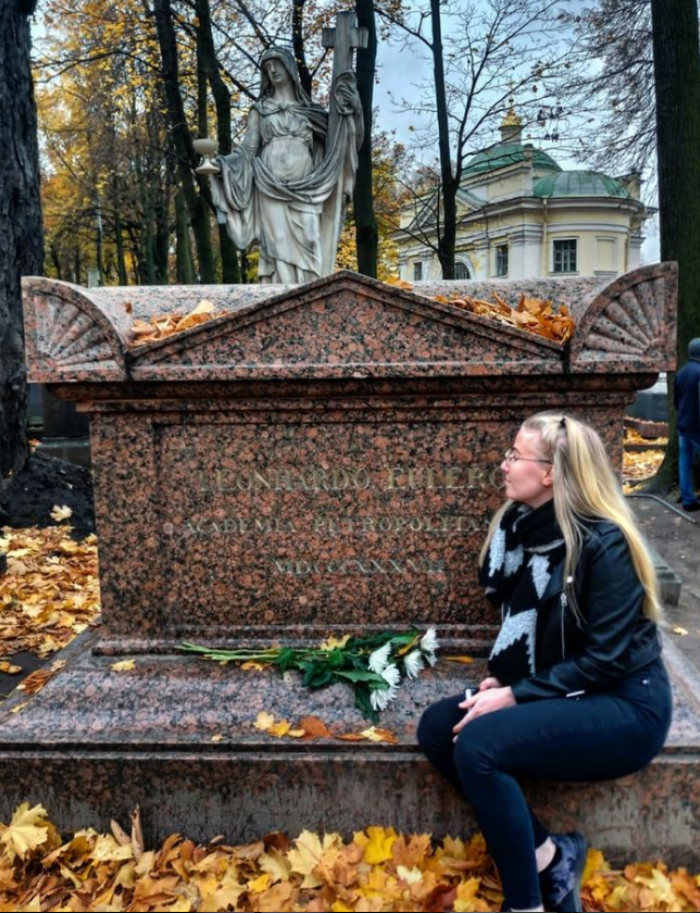
\includegraphics[scale=0.6]{eulerinhauta.png}
\label{hauta}
\caption{Eulerin haudalla Pietarissa syksyllä 2019.}
\end{figure}
 
\newpage

\nocite{*}
\printbibliography
 

 
\end{document}